% !TEX root = main.tex
\chapter{Construction}
\label{chap:construction}

  This chapter concerns the construction of the rear wing. The step from theoretical abstraction to a real product. This includes dimensioning, material selection and finalizing the wing. The simulated rear wing lacks a proper mounting method, as the design depends on the external group at Vermilion Racing.

\section{Requirements}

  The formula student competition has a clear ruleset dictating the strength requirements of aerodynamic devices. The most crucial elements are outlined below:

  \subsection{Strength Requirements}

    The competition rules set up strength requirements for the aerodynamic devices, making sure wobbling or unsafe structures are prohibited. The rules are seen below:

    \begin{tcolorbox}[colframe=seapurple,colback=seapurple!1]
      Aerodynamic Devices Stability and Strength:
      \begin{itemize}
        \item [T7.5.1] Any aerodynamic device must be able to withstand a force of $\SI{200}{\newton}$ distributed over a minimum surface of $\SI{225}{\centi\metre\squared}$ and not deflect more than $\SI{10}{\milli\metre}$ in the load carrying direction.
        \item [T7.5.2] Any aerodynamic device must be able to withstand a force of $\SI{50}{\newton}$ applied in any direction at any point and not deflect more than $\SI{25}{\milli\metre}$.
      \end{itemize}
      \vspace{5pt}
      \hspace*{\fill}\tiny{Rules from Formula Student UK 2018 ruleset \cite{FSrules18}.}
    \end{tcolorbox}

    Thus, deflection of the wing has to be calculated, in order to comply with the rules.

\section{Material Selection}

  Selecting a fitting material depends on the maximum deformation and weight. According to the PDS (see section \ref{sec:PDS}), the wing has to be \emph{as light as possible} in order not to move the center of mass further upwards. Furthermore, it needs a high \emph{elastic modulus} in order to be stiff as to not deform by aerodynamic forces. The wing needs to be have a \emph{high yield strength}, be \emph{low cost} and easy to produce time wise.

  Drawing on experience from competitors, carbon fiber- and glass fiber reinforced polymers are the weapons of choice \cite{FSwingmaterial}. However, Cambridge Engineering Selector, a material selection tool was used in order not to leave a stone unturned. The results can be seen in figure \ref{fig:CESmatchoice}, where materials of high elastic modulus are plotted against their density. Magnesium and some aluminium alloys are near the carbon fiber reinforced polymers, but machining an entire wing out of metal is incredibly time consuming and expensive. Carbon fiber reinforced polymers are chosen as a material, and the next chapter will investigate the properties and strength of the composite structure.

  \begin{figure}
    \makebox[\textwidth][c]{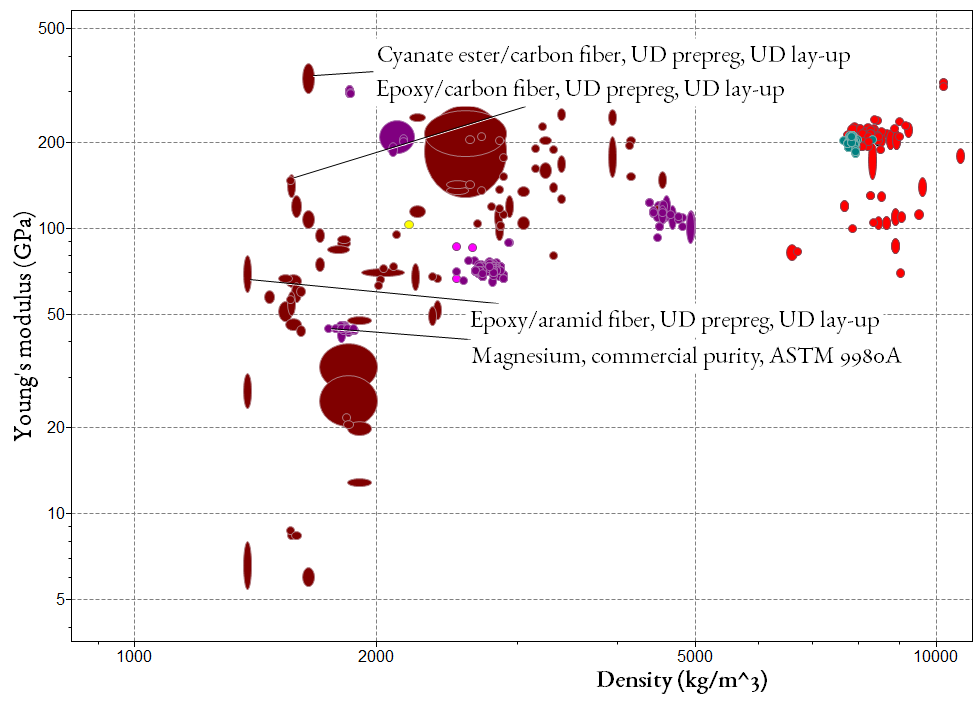
\includegraphics[width=1.2\textwidth]{CESmatchoicegood}}
    \caption{Cambridge Engineering Selector (CES) showing the various aerospace grade materials usable for this application. The dark red dots are compositites, while the dark purple dots are metals such as aluminium and magnesium.}
    \label{fig:CESmatchoice}
  \end{figure}

\section{Composites}

  The geometrical shape of a composite structure can be highly varied, which can increase strength dramatically. The second moment of inertia of a simple beam can be increased by moving material from the neutral axis, as is done in a standard I-beam. The same thing applies to composites: A soft, but light core can be added with a hard shell (in this case carbon fiber) surrounding the core.

  An approximation of the wing profile is a box shape, where the moment of inertia is much easier calculated. From \cite{DIAB}, the strength of the sandwich material can be mathematically described as:
  \begin{align}
    D &= EI = E_{cs} \frac{bh^3 - ec^3}{12} + E_c \frac{ec^3}{12}
  \end{align}
  Where $E_cs$ is the elastic modulus of the composite shell, $E_c$ is the elastic modulus of the core, $b$ is the width of the beam, $h$ is the height of the beam, $e$ is the width of the core and $c$ is the height of the core.
  The strength of a fiber composite depends on the fiber direction, the relationship between the fiber and matrix, and the porosity of the composite. The load bearing properties in the fiber direction is given by:
  \begin{align}
    E_\text{long} &= E_f \text{Vol}_{f\%} + E_m (1-\text{Vol}_{f\%} )
    \intertext{Where $E_f$ is the elastic module of the fiber and $E_m$ is the elastic modulus of the matrix. The $\text{Vol}_{f\%}$ is the fiber volume fraction of the composite. For a transverse load, which is what rule T7.5.1 and T7.5.2, the strength of the sandwich construction is found as:}
    \frac{1}{E_\text{transverse}} &= \frac{\text{Vol}_{f\%}}{E_f} + \left( 1 - \frac{\text{Vol}_{f\%}}{E_m}\right)
  \end{align}
  For the biaxial carbon fiber weave used in this construction, the strength is almost $50\%$ less in the transverse direction \cite{DIAB}. The effective elastic modulus is found to be $\approx \SI{60}{\giga\pascal}$. Using the beam approximation that the deflection of the rear wing functions as a beam with a core supported in both ends is found to be: \cite{tekniskstabi}

  \begin{align}
    \delta_\text{max} &= \frac{PL^3}{192EI} = \SI{0.03}{\milli\metre}
  \end{align}

  Which is far below the maximum allowed by a factor of more than $300$. This also ensures the wing keeps its dimensions even though a high downforce is present.

\section{Final Design of Rear Wing}

\begin{figure}
  \makebox[\textwidth][c]{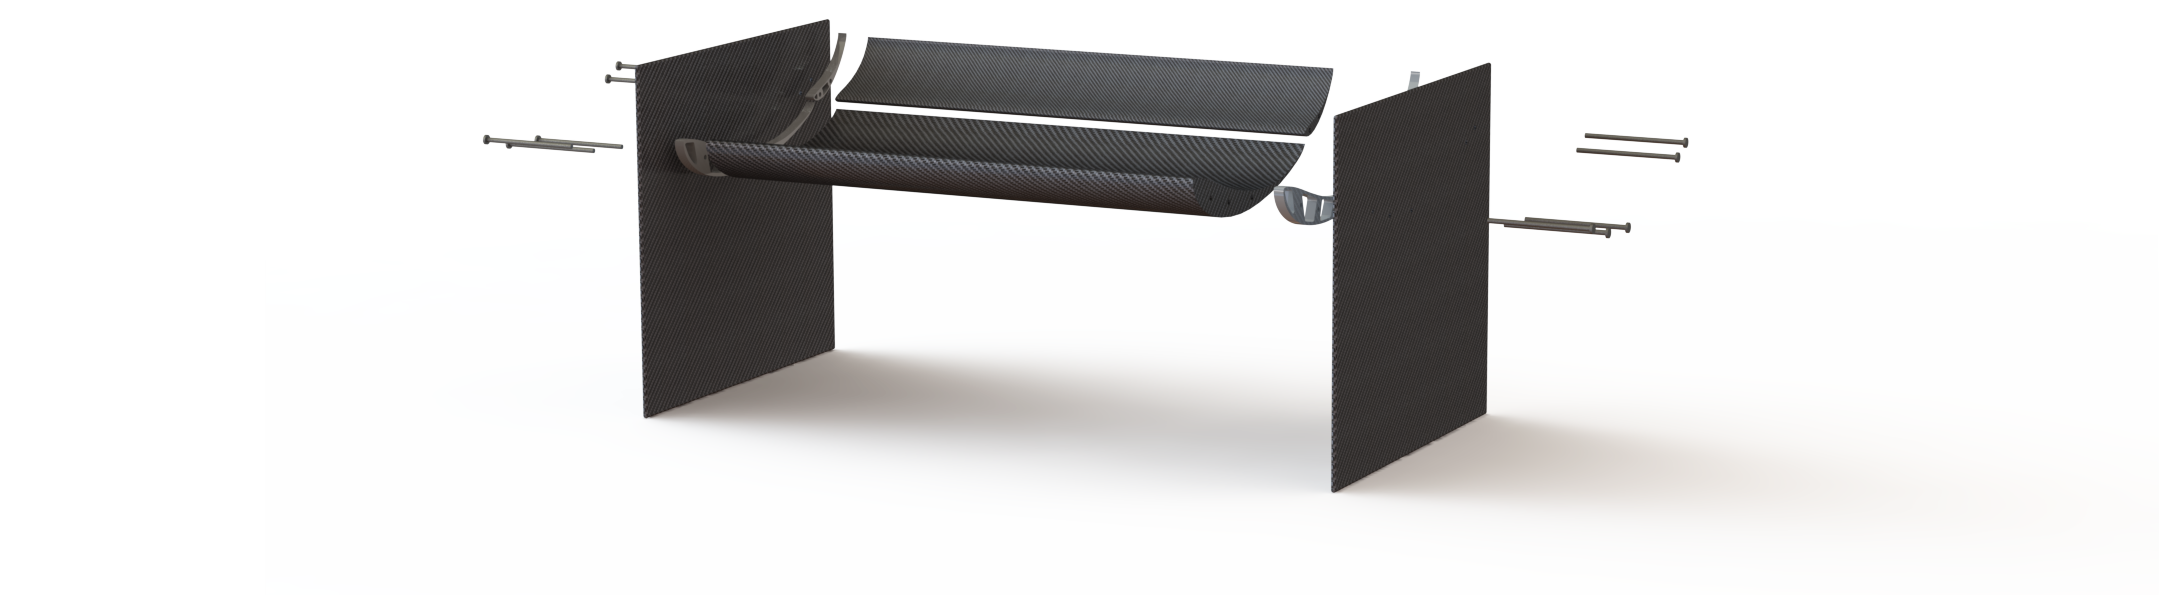
\includegraphics[width=2.4\textwidth]{finaldesignrender3}}
  \caption{Render of the final design of the rear wing in exploded view.}
  \label{fig:finaldesignrender}
\end{figure}

  Designing the final design can be done based on the investigations produced in the previous chapters. First, the FSUK rules restrict the cross sectional dimensions, as seen in figure \ref{fig:cadplacement}. Thereto, the rule \emph{T7.3.2   All aerodynamic devices higher than 500 mm from the ground, must not extend outboard of the most inboard point of the rear wheel/tire} dictates the width of the wing. According to the car's current design, the inner dimension from wheel to wheel is $\SI{1100}{\milli\metre}$, and thus serves as the maximum width of the wing.

  The two elements of the full scale wing will be bolted to the endplates at the optimal found angle of attack. The wing elements will have two metal brackets glued to the inside of the carbon fiber wings, the bracket will be have holes with M10 threads in which the endplates are bolted to secure the structure. The structure can be seen in figure \ref{fig:finaldesignrender}, with end plates, brackets, wings and bolts.

  \subsection{Topology Optimization of Wing Brackets}

  In order to minimise the weight of the metal bracket inserts topology optimizations where made using the build in function in \emph{Fusion 360}, in which all simulations are done in the cloud. Topology optimization tries to reduce the weight of the model by removing excess material while maintaining stiffness and strength of the model.

  The inserts were modeled from the wing profile and the location of the inner threads was chosen. The model was then meshed with a target cell size of $\SI{1.5}{\milli\metre}$, and the target weight reduction was set to $70\%$, with a downforce load of $\SI{250}{\newton}$ at the surface.

  \begin{figure}
    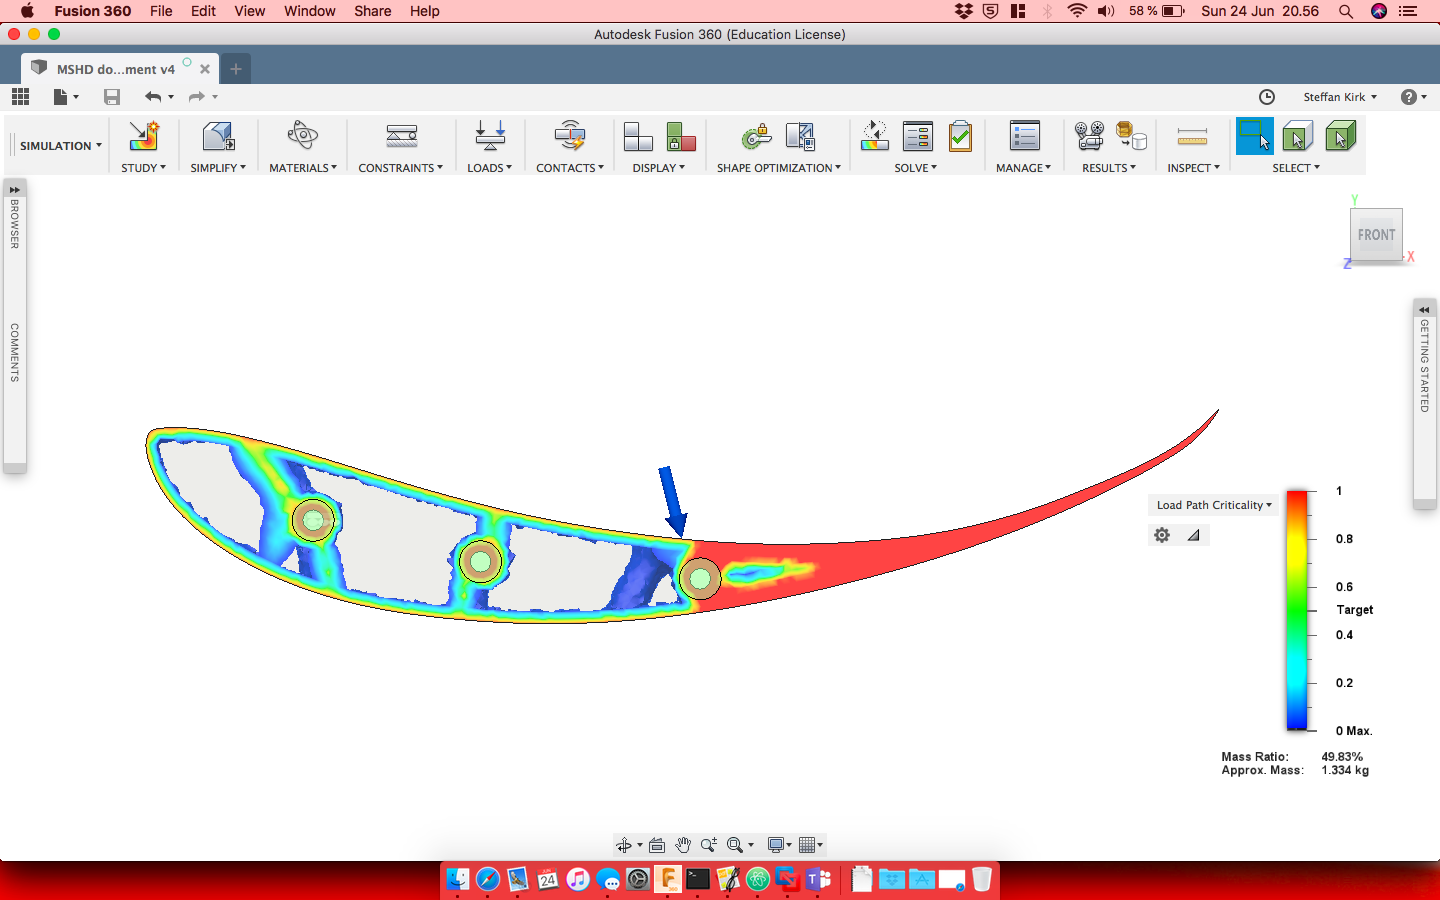
\includegraphics[width=\textwidth]{Optimisedlargewinginsert}
    \caption{The result of the topology optimization for the large insert, with a weight reduction at about $\SI{50}{\%}$.}
    \label{fig:topology_large_insert}
  \end{figure}

  The result of the optimization for the large insert is shown in figure \ref{fig:topology_large_insert}, was then used to remove excess material from the model. The results were overlayed on the model and material could be cut from the original model as shown in figure
  \ref{fig:meshoverlay}. The final model of the large insert was then created with a weight reduction around $\SI{40}{\%}$. A render of the final model is shown in
  figure \ref{fig:render_large_insert}. The same procedure was done for the smaller metal wing insert, and technical drawings of are included in following section. \fxnote{Not there. Where should they be?}

  \begin{figure}
    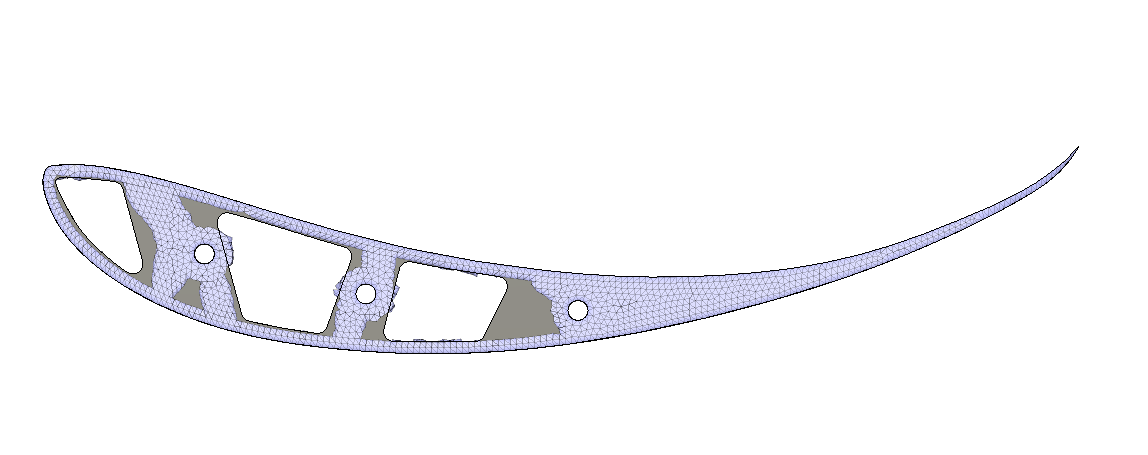
\includegraphics[width=\textwidth]{meshoverlayedlargeinsert}
    \caption{Optimized mesh overlayed on model so excess material could be easily removed.}
    \label{fig:meshoverlay}
  \end{figure}

  \begin{figure}
    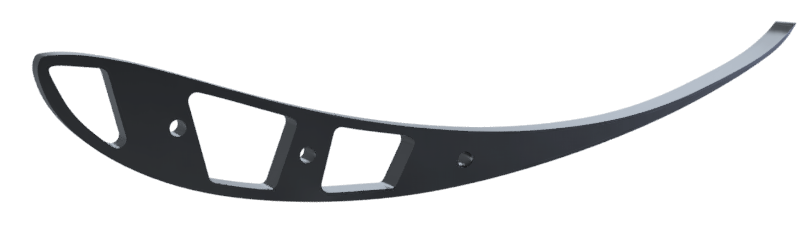
\includegraphics[width=\textwidth]{largeinsertrender}
    \caption{Render of the final model for the metal insert, with a weight reduction around $\SI{40}{\%}$.}
    \label{fig:render_large_insert}
  \end{figure}

  The two elements of the full scale wing will be bolted to the end plates at optimal found angle of attack. The wing elements will have two metal brackets glued to the inside of the carbon fiber, the bracket will be have holes with M10 threads in which the endplates are bolted to secure the structure.

\section{Manufacturing Final Design}

  The following section describes the steps required to build the wing physically. First, templates of the MSHD airfoil are lasercut. The templates are mounted on the sides of polystyrene blocks, where a homemade hot wire cutter cuts the foam cores of the wing. The foam cores are then glued together into the appropriate lengths, where the carbon fiber mattes are draped over. The carbon fiber is then reinforced by an epoxy resin, which over a 24 hour period is hardened. The surface is then polished, and finally resealed by adding another layer of epoxy resin. The wing is then bolted to the end plates through the two metal brackets inserted into the wing's ends.

  \subsection{Polystyrene Molds}

  \begin{figure}
    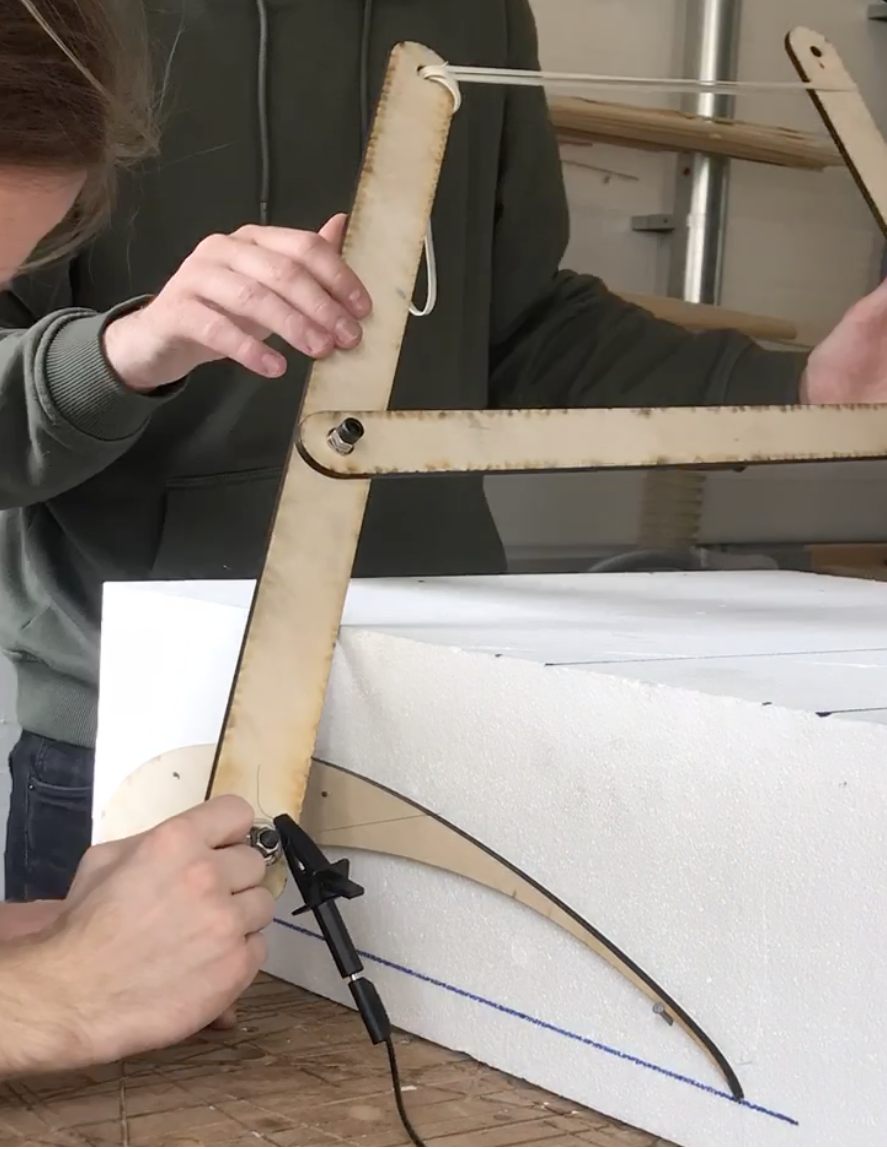
\includegraphics[width=\textwidth]{hotwiremethod}
    \caption{The hot wire melts the styrofoam while sliding along the wooden template.}
    \label{fig:hotwire}
  \end{figure}

  The molds for the wings were chosen as positive molds, meaning polystyrene molds of the actual wings were cut out and overlaid with resin coated carbon fiber. In order to do this, we devised a hot wire-based specialized tool for the job. This can be seen in figure \ref{fig:hotwire}, where a $\SI{0.3}{\milli\metre}$ heat resistant
   wire was used at $\SI{12}{\volt}$ drawing $\SI{2.5}{\ampere}$ over a cutting length of $\SI{600}{\milli\metre}$. In order to get the correct airfoil shapes, the MSHD airfoil profile was lasercut out of 3mm plywood. The wooden profile is then mounted on the sides of the polystyrene block, where the hotwire is pulled across in a timely fashion. In order to produce a smooth surface, two people have to move very coordinated. Going too slow leaves deep melting lines, and moving too fast makes the hotwire ''slack'' in the middle as it does not have enough energy to melt the polystyrene quick enough, causing the airfoil profile to be skewed.

  All hotwire cutting was done by hand over several days, and we owe a special thanks to our sponsor DTU Skylab for providing the polystyrene blocks.

  \subsection{Hand Layup}

    \begin{figure}
      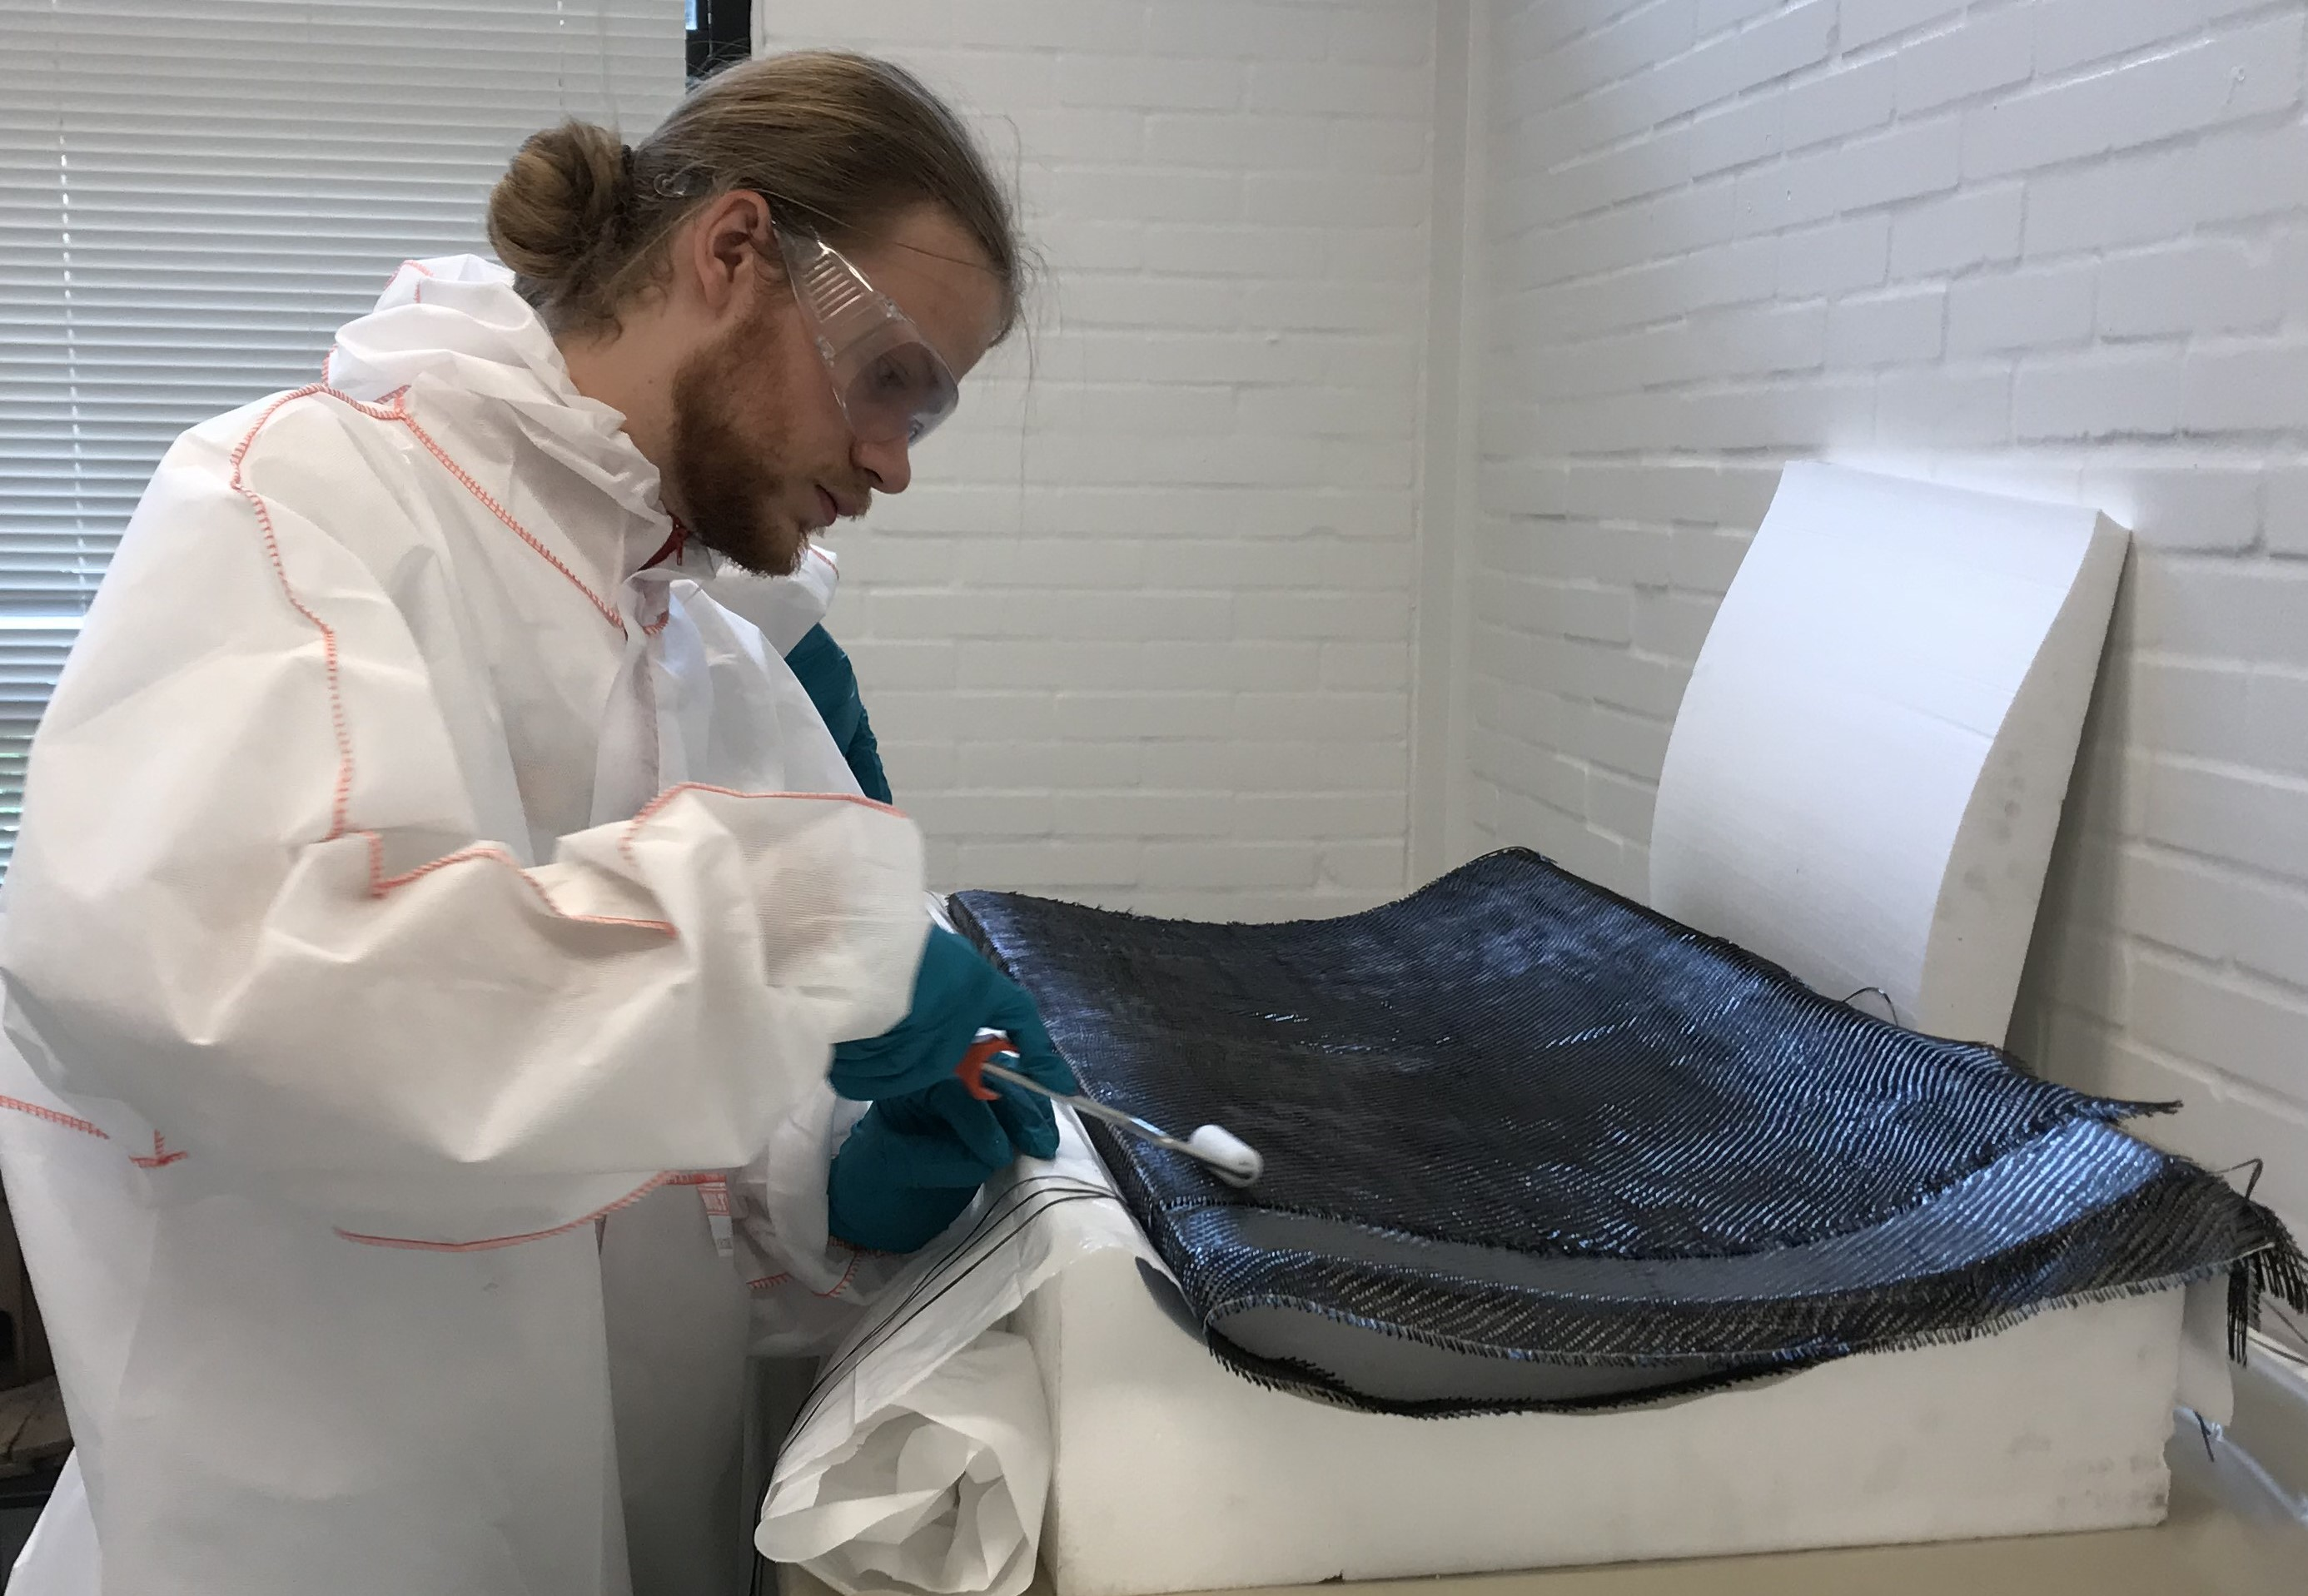
\includegraphics[width=\textwidth]{handlayupwnicolai}
      \caption{Steffan and Nicolai performing a hand layup of the carbon fiber mats around a polystyrene foam core.}
      \label{fig:handlayup}
    \end{figure}

    The finished positive molds are used both as molds where carbon fiber is applied on, as well as foam cores that reinforce the structure. The molds are then placed inside the negative forms of the molds, where carbon fiber is draped over the surface. The epoxy is then applied to the carbon fiber matte by a soft brush, and air is rolled out by spiked rollers. Nicolai Boertman is seen performing this action in figure \ref{fig:handlayup}, putting the final layer on the main element of the rear wing. The white polystyrene mold underneath the carbon fiber is the negative mold, which helps keep the shape when applying to carbon fiber to the other side. After rolling out the epoxy satisfyingly, a plastic tarp is added to the surface and rolled down neatly without air bubbles. This ensures getting a smooth surface, and lets the wing cure in a closed environment.

    \begin{figure}
      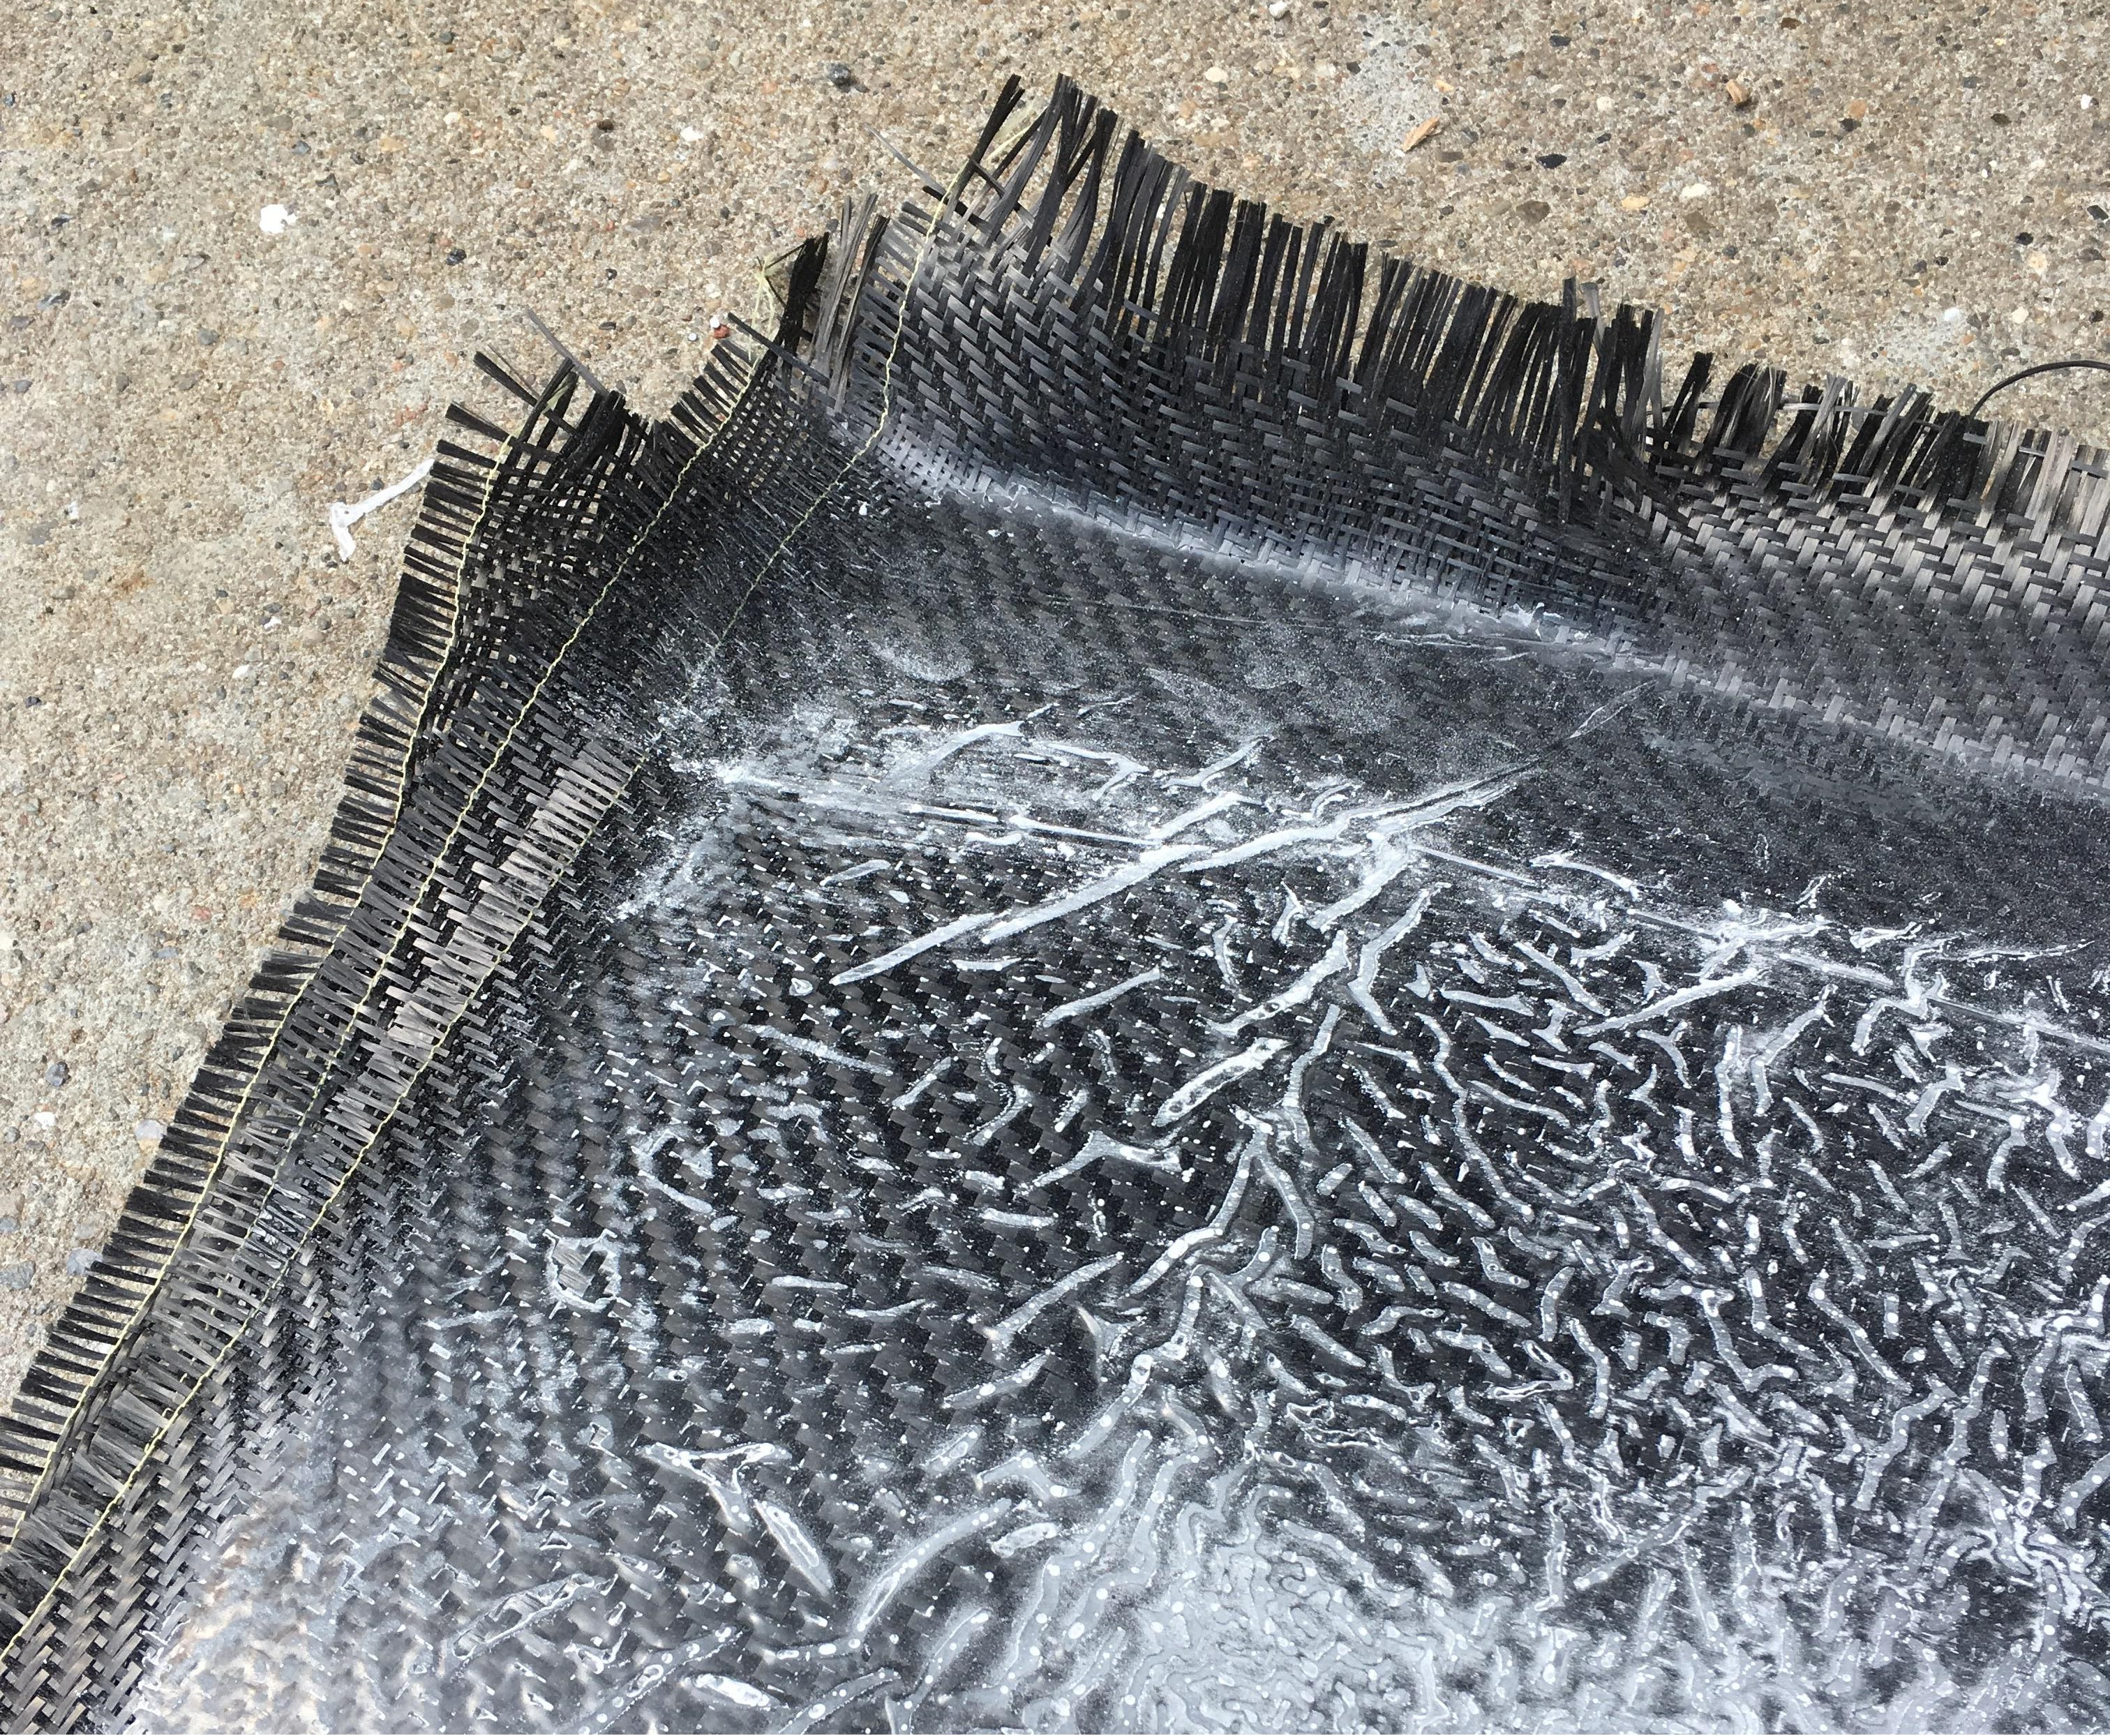
\includegraphics[width=\textwidth]{residualepoxy}
      \caption{Curing the wing in a flat position lets the resin pool in the center of the wing. This causes the surface to be very rough, potentially causing the boundary layer to trip early. A very unwanted effect that requires mending.}
      \label{fig:roughsurface}
    \end{figure}

    Three methods of curing was attempted:

    \emph{The wing hanging freely with no pressure}: The results was good. No pooling of epoxy, the surface was relatively smooth, but an additional sealing layer had to be applied, as the epoxy had been displaced from the surface. This gave it the surface roughness of the fibers, which is not optimal.\newline
    \emph{The wing laying flat under pressure with the convex shape pointing upwards}: This was highly successful, giving a very smooth surface with the right amount of epoxy covering it. No additional treatment was required.\newline
    \emph{The concave shape pointing upwards}: The results was not good, but workable. The results can be seen in figure \ref{fig:roughsurface}. The epoxy pooled due to gravity forcing the epoxy down towards the center of the cambered wing. Getting a proper surface finish from this is handled in the section below.

  \subsection{Surface Finish}

    Curing \emph{should} occur by securing the wing \emph{vertically} or with the convex shape pointing upwards, as to not let epoxy pool up on the concave surfaces. This knowledge was forgotten on one of the wings, as seen in figure \ref{fig:roughsurface}, where the surface has become very rough due to epoxy pooling. Albeit not optimal, the wing can be salvaged by sanding. The finished product after sanding and preparing the surface is shown in figure \ref{fig:wingaftersanding}. The surface finish is done with a thin layer of extra epoxy. Using a clear lacquer was also investigated, but the reduced durability of the lacquer is not optimal \cite{lacquersucks}. The wing has to survive transport to England, which can damage a soft surface.

    \begin{figure}
      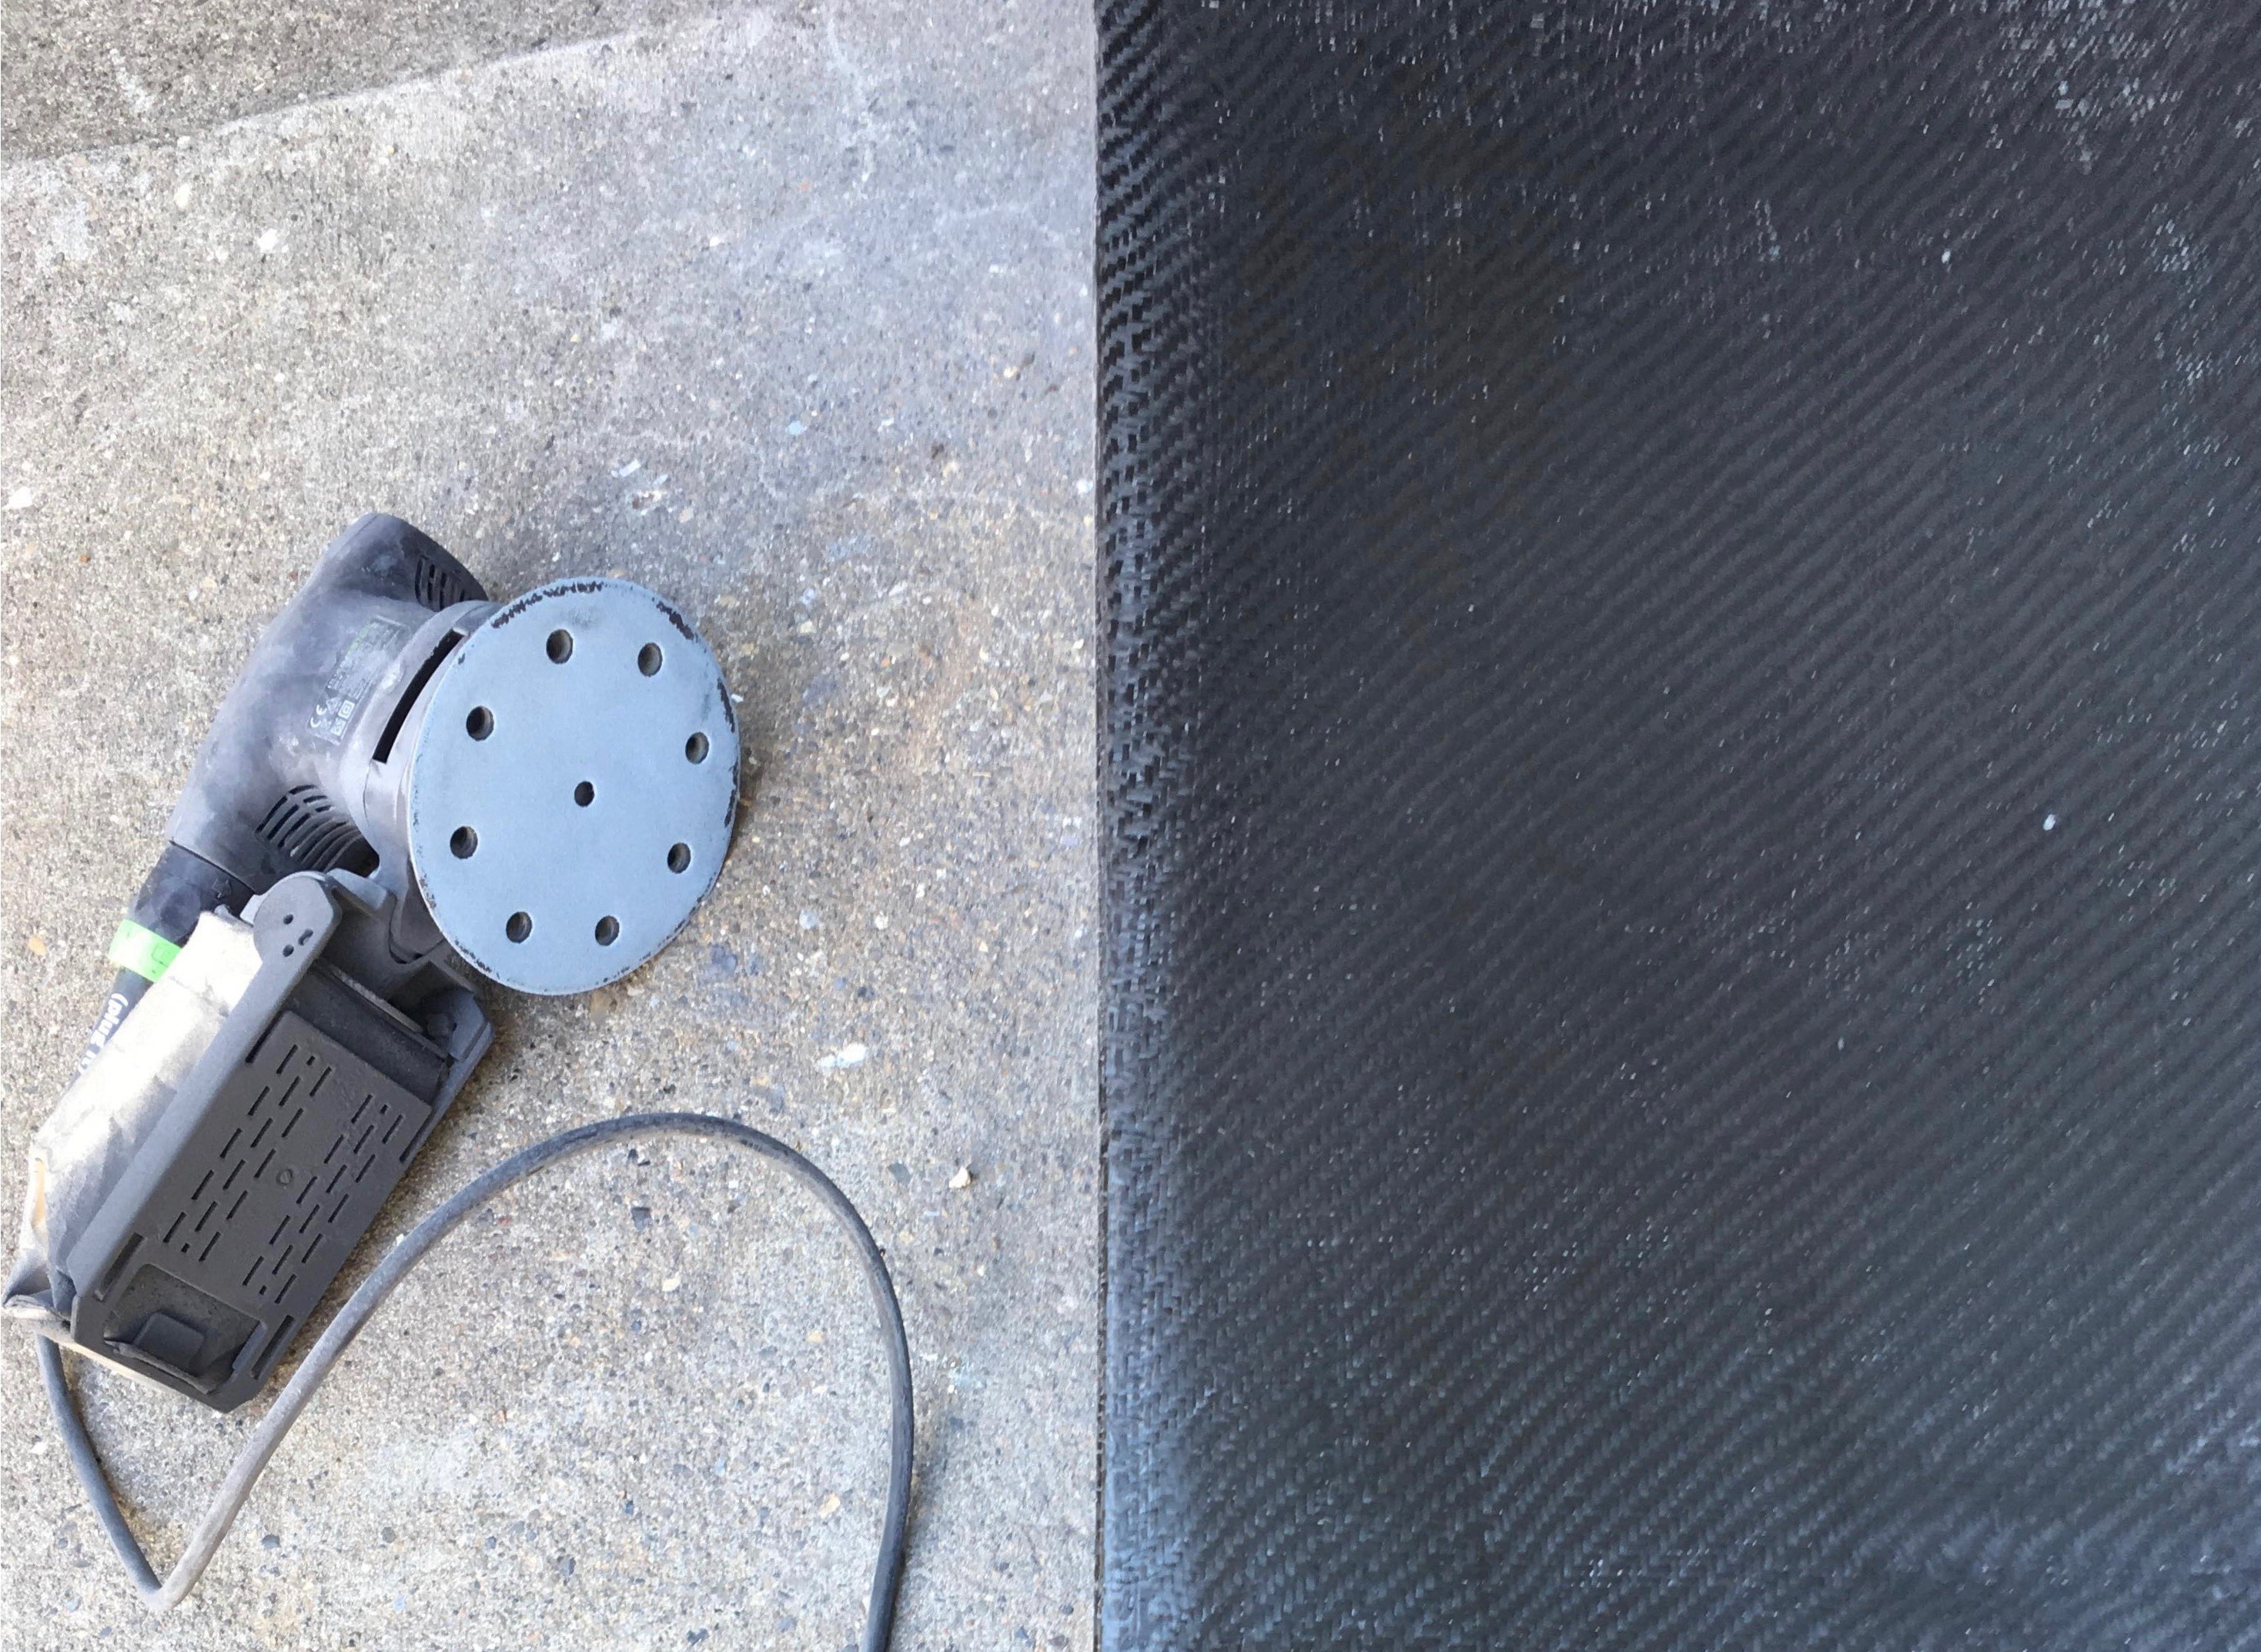
\includegraphics[width=\textwidth]{wingaftersandingperfect}
      \caption{Sanding the wing clears the surface roughness, but requires a new layer of sealant. Using epoxy or a lacquer was investigated before settling on epoxy.}
      \label{fig:wingaftersanding}
    \end{figure}

  \section{Final Assembly}

    The final assembly of the wing is going to be done in July before competition start. A complete design of the wing is not feasable at this stage, due to many unforeseen changes in how the rear of the car is going to fit together. The wing is not essential for a bare minimum product, which is why the fitting herof is not a priority for the team as a whole.
